% vim:set ft=tex:
\section{Fiasco.OC \& L4Re}
\label{state:env}
The related research presented in section \ref{state:related} states
requirements of kernel features:
hardware performance counters, assignment of threads to specific
cores, and the ability to overrule the kernel scheduler.

Fiasco.OC is a µ-kernel of the L4-family and follows the design paradigm to
only implement mechanisms in the kernel and no policies.
For performance reasons the scheduling policy is the only policy implemented in
the kernel.
The scheduling parameters in a scheduling request form user land consist of
a priority level, a time slice size request and a descriptor on which cores the
thread wants to be scheduled.
The kernel selects the first available core from the descriptor to schedule the
thread on, checks if the priority level is in a valid range, and assigns a time
quantum.
It does neither balance the amount of threads per core, nor prevent
oversubscription of one core.
However, it provides the mechanism to design a more sophisticated load
distribution scheme as user level service.

Regarding hardware performance counters, the kernel provides neither a system
call interface to read or configure them, nor per thread accounting of
configured counters.
Access to hardware performance counters is critical for this project, so a
mechanism has to be provided for a user level service.

The L4 Runtime environment provides a scheduling service skeleton, which
defines the kernel and user interface.
Using this skeleton the service can replace the default L4Re scheduler and do
more analysis of each thread.
This skeleton also enables thread specific proxies with an individual
configuration.

\begin{comment}
\textbf{Fiasco.OC}
\begin{itemize}
  \item Kernel scheduler does no balancing, assigns thread to the first
    core specified in the affinity descriptor
  \item affinity descriptor: core(s) a thread should run on
  \item Syscall via run\_thread() to pass affinity descr to kernel scheduler
  \item interface to query execution time for each thread
  \item capability system -- to derive communication relationships from
  \item	Kernel feature wishes derived from related work: Performance counters
    and per thread accounting
\end{itemize}

\textbf{L4Re}
\begin{itemize}
  \item provides scheduler proxy interface, including affinity descriptor,
    scheduling parameters
  \item syscall interface
\end{itemize}
\end{comment}


% -----------------------------------------------------------------------------

\section{\gls{intel} Haswell Architecture}
\label{state:haswell}

In section \ref{state:related} several hardware features were mentioned.
The most important of all are performance counters for cache misses, cycles and
instructions executed.
Those and many more are present in the target processor: an \gls{intel} Core
i7-6440K.
The processor has ``architectural performance monitoring version 3''
capabilities, which consists among other features of three fixed-function
performance counters counting Instruction Retired, Unhalted Core Cycles, and
Reference Instruction Retired.
In contrast to the first two counters, the last counter is unaffected by
processor speed changes due to power saving or turbo boost features.
Besides these, four general purpose performance counters are available per
logical core, which can be programmed to count one specific event.
All \gls{intel} Core i generations support architectural performance monitoring
in different versions, but all versions are guaranteed to support the events
listed in table \ref{state:table:core_events}: Unhalted Core Cycles,
Instruction Retired, Unhalted Reference Cycles, LLC Reference, LLC Misses,
Branch Instruction Retired, and Branch Misses Retired.

Besides these central events, each hardware generation supports a different set
of so called ``non-architectural performance events''.
This non-architectural event set allows to monitor many specific events, e.g.
L2-misses/-hits, micro-ops per logical core executed per cycle, or unhalted
core cycles, while the logical core is in ring 0.

Another difference to the target processor, compared to most processors used in
earlier research is the \gls{smp} architecture. In contrast to \gls{cmp}
architectures no cache groups are defined by the hardware, because the
\gls{llc} is shared among all cores.
Figure \ref{state:fig:core_layout} shows examplary the cache hierarchy and core
components of the \gls{intel} Haswell processor.
Each core consists of two \gls{ht} cores, sharing L1- and L2-caches.
Besides the \gls{llc} the cores on one socket share nothing.
The caches are inclusive, meaning each cache line present in L1I or L1D
cache is also present in the corresponding L2 cache and each L2 cache line is
also present in the \gls{llc}.
This eases the lookup of cache lines in other cores on the same package.

%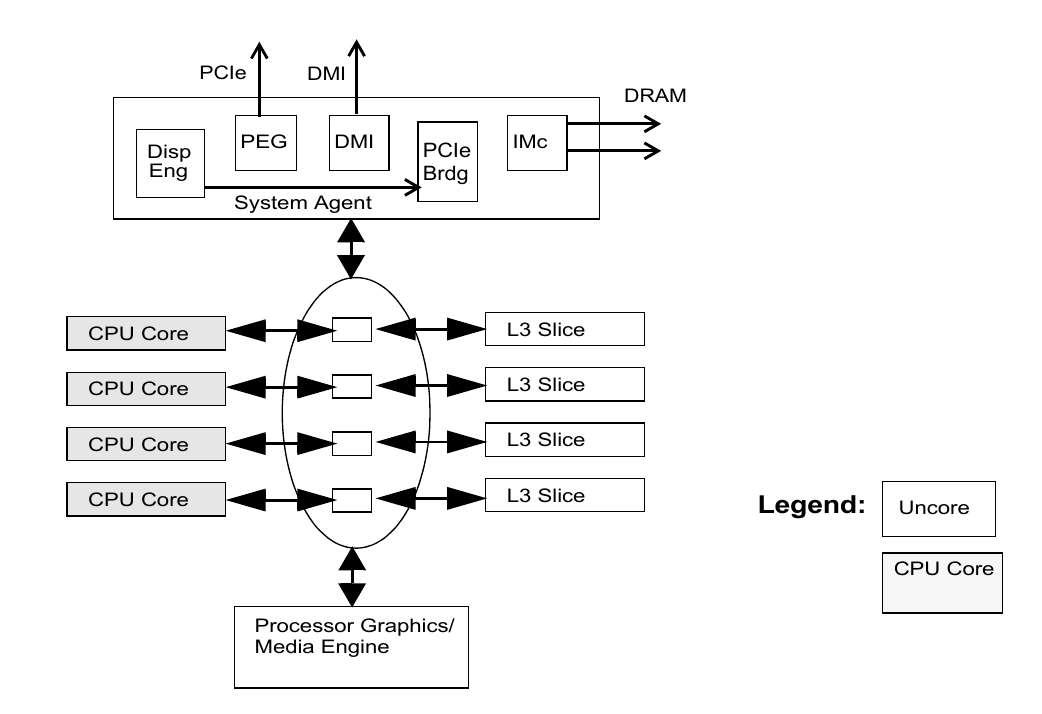
\includegraphics[width=0.8\textwidth]{images/haswell_architecture_by_intel_large}

\begin{figure}[h!]
  \centering
  \includegraphics[width=0.7\textwidth]{images/haswell_core_layout}
  \caption{Layout of a Core i7-4660K quad-core.
    Each physical core has two logical cores T0 and T1 sharing the cores L1I-,
    L1D-, and L2-cache.}
  \label{state:fig:core_layout}
\end{figure}

\begin{comment}
\begin{itemize}
  \item diagram of architecture: four cores with L1I/D \& L2 cache; two smt/ht
    cores per physical core; L3 cache shared and sliced, ring buffer for
    access; mem controler in uncore package;
  \item 4 prefetcher per cache; 2 for L1D, 2 for L2 cache
  \item L1D \& L2 cache data is present in L3 cache to be able to redirect
    requests from other cores to the correct cache. --> Issue with security; no
    cache side attack surface reduction
  \item IF security: dual socket system with one core dedicated to security
    tasks for an interval
  \item L3 cache slices corespond to number of cores
  \item logic portion and data array portion; access, coherency, memory
    ordering, LLC misses, writeback to memory; cache lines
  \item hash function uniformly distributes addresses
  \item access times to L3 cache varies depending on travel distance on the
    bi-directional ring buffer
  \item system agent receives memory requests not serviced by cache and
    redirects to IMC
\end{itemize}
\end{comment}

% -----------------------------------------------------------------------------
